\documentclass{article}

%% Page Margins %%
\usepackage{geometry}
\geometry{
    top = 0.75in,
    bottom = 0.75in,
    right = 0.75in,
    left = 0.75in,
}

\usepackage{amsmath}
\usepackage{graphicx}
\usepackage{parskip}

\title{Assembly Project: Breakout}

% TODO: Enter your name
\author{Frederick Meneses & Name 2}

\begin{document}
\maketitle

\section{Instruction and Summary}

\begin{enumerate}

    \item Which milestones were implemented? 
    % TODO: List the milestone(s) and in the case of 
    %       Milestones 4 & 5, list what features you 
    %       implemented, sorted into easy and hard 
    %       categories.
    Milestones 1-5 were implemented. 
    
    Easy: Player can launch the ball at the beginning of each attempt.
    
    Hard: Player score is tracked by how many bricks have been broken on the bottom left with green pixels. 
    
    Bricks require multiple hits to be broken. Orange bricks require 3 hits, Purple bricks require 2 hits, Cyan bricks require 1 hit. 
    
    Lastly, the direction/speed of the ball changes based on the collision with the paddle. In the center, it bounces straight up. The bounce angle is more pronounced at the edges of the paddle. The first angle makes the ball go (1, 2) units in any direction. The sharper angle makes the ball go (1, 1) units in any direction.
    
    \item How to view the game:
    % TODO: specify the pixes/unit, width and height of 
    %       your game, etc.  NOTE: list these details in
    %       the header of your breakout.asm file too!
    
    \begin{enumerate}

    \item	4 pixels/unit
    \item	128 pixel width
    \item	128 pixel height
    \item Controls: Space (launch ball), h (paddle left), l (paddle right)

    \end{enumerate}

    
\begin{figure}[ht!]
    \centering
    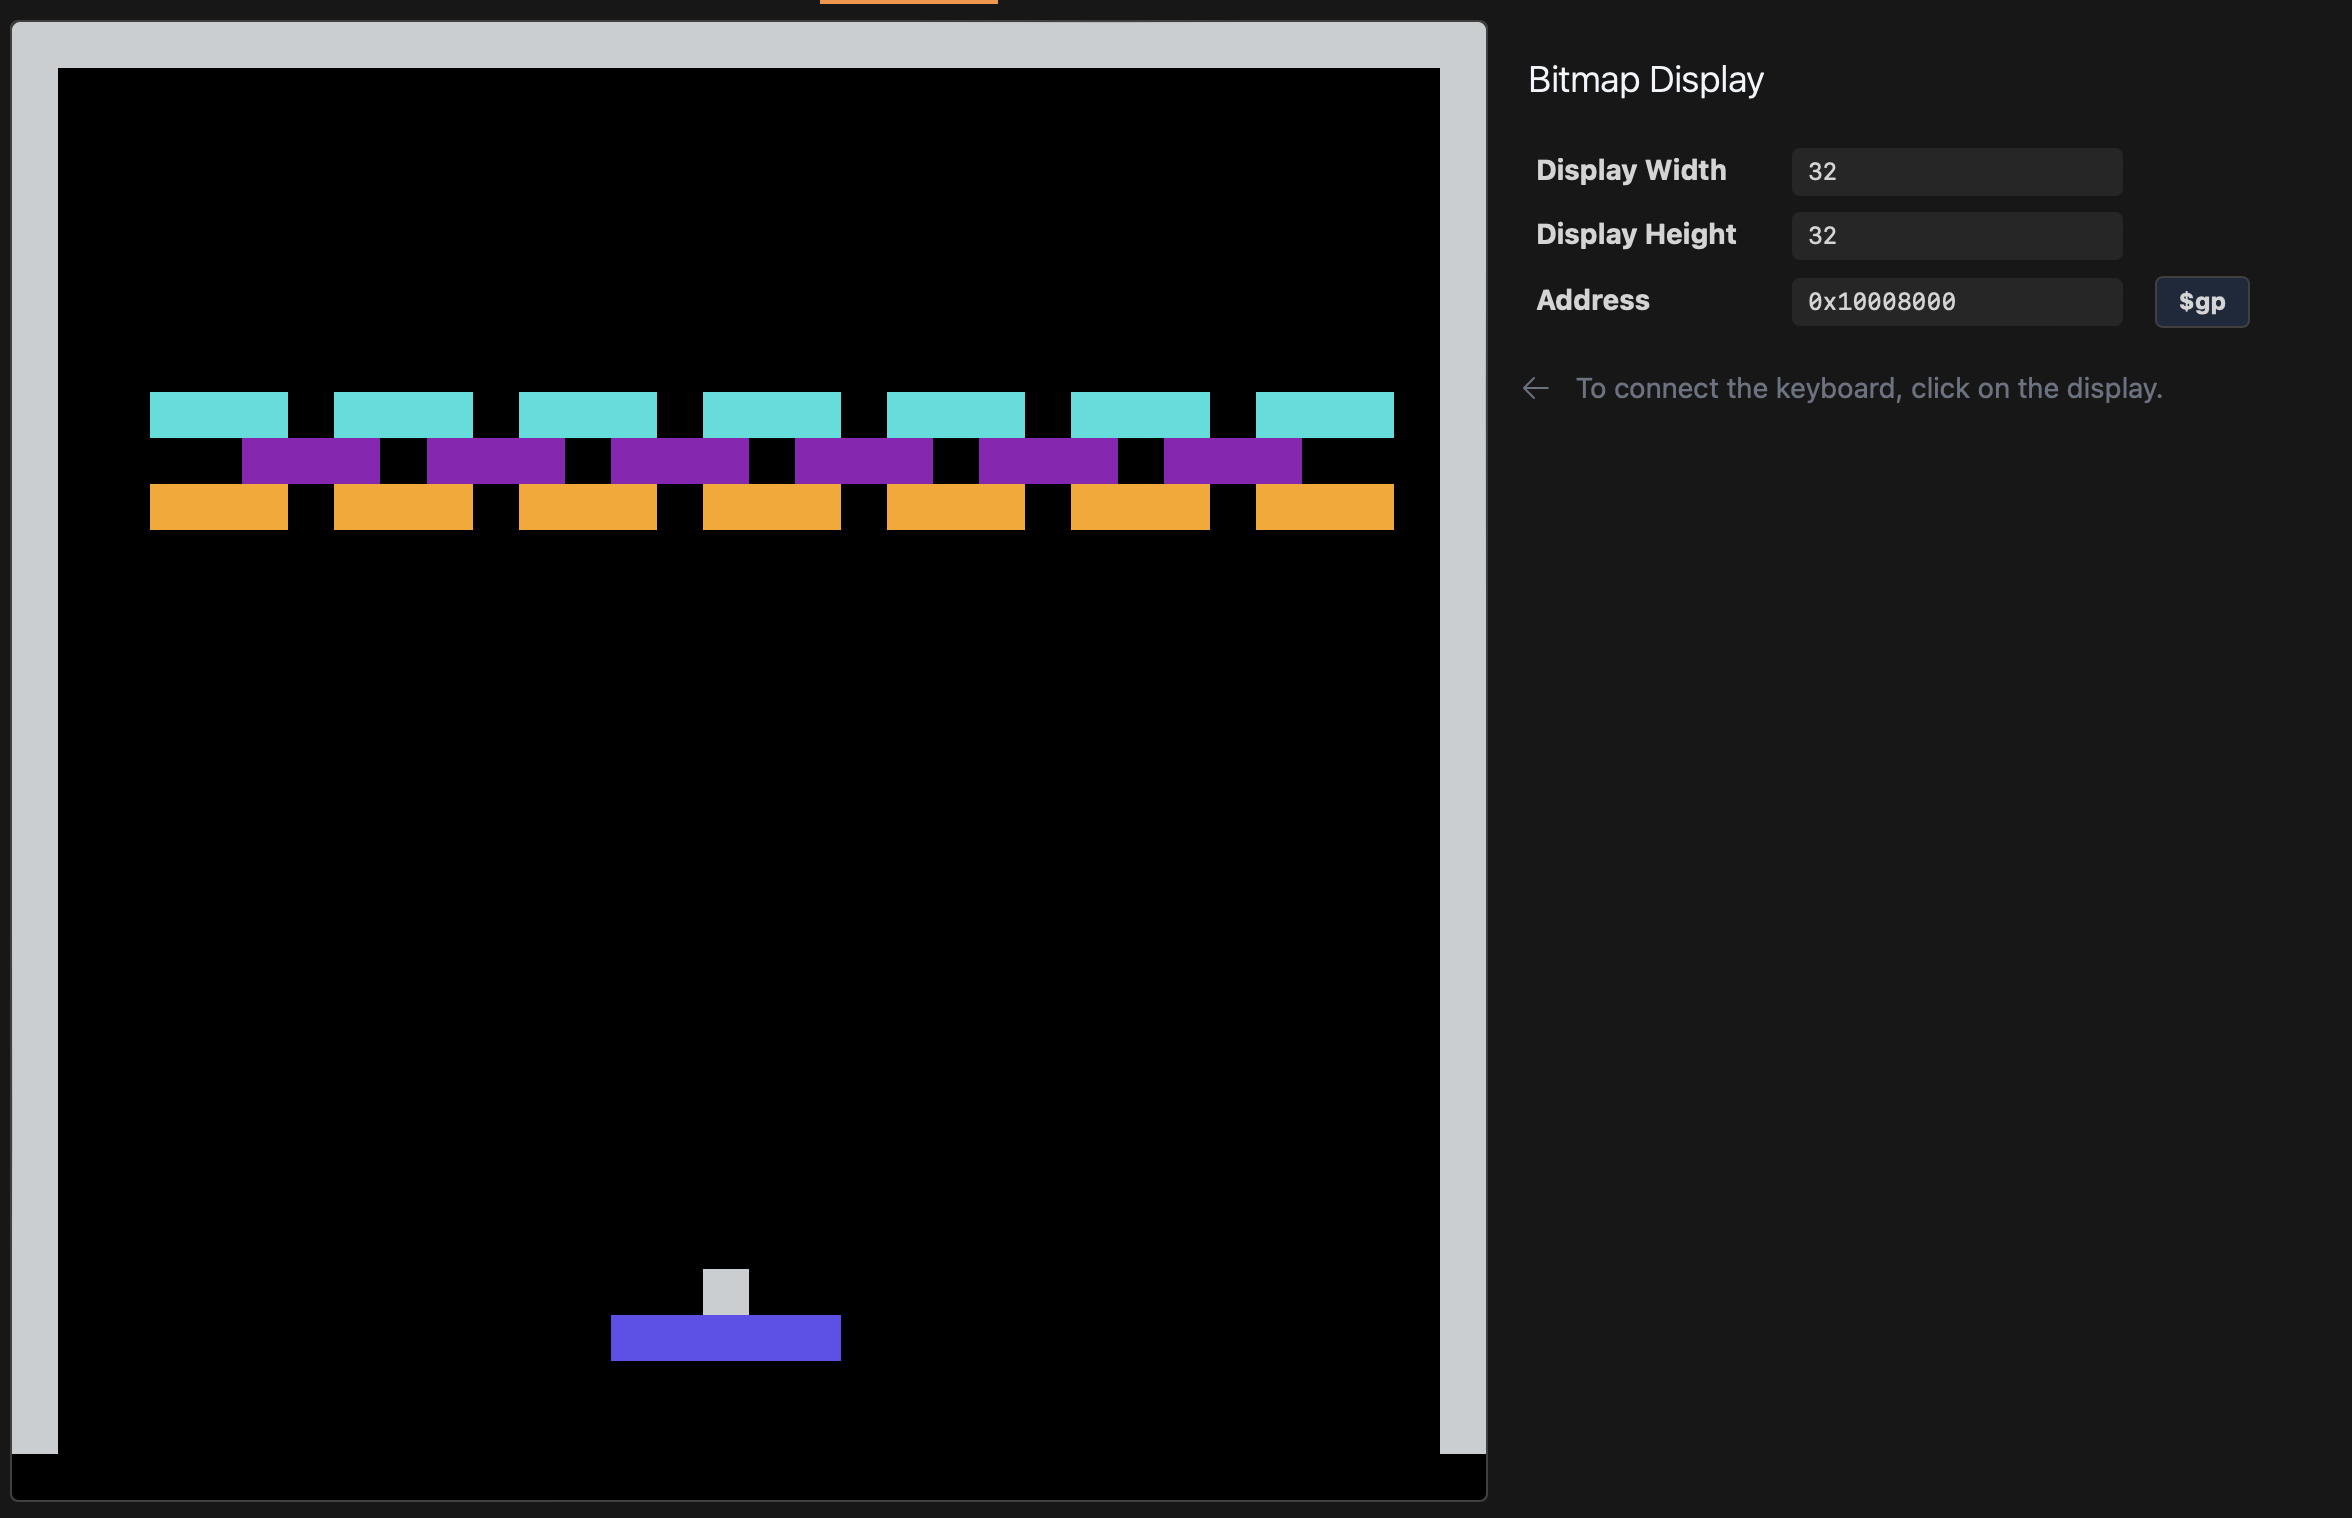
\includegraphics[width=0.6\textwidth]{static.png}
    \caption{Static Background}
    \label{Static}
\end{figure}

\begin{figure}[ht!]
    \centering
    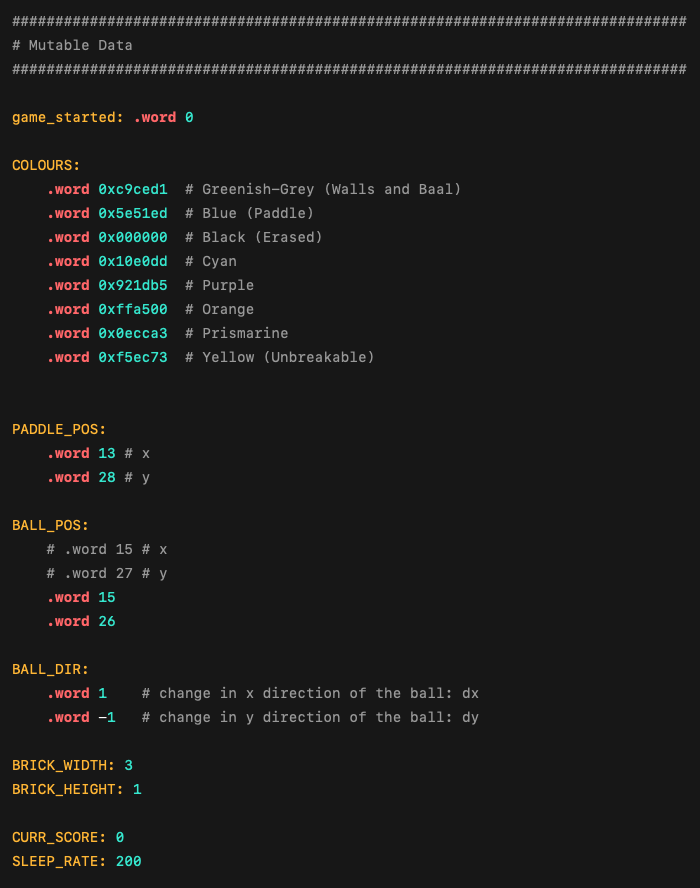
\includegraphics[width=0.6\textwidth]{memory.png}
    \caption{Memory}
    \label{Memory}
\end{figure}

\begin{figure}[ht!]
    \centering
    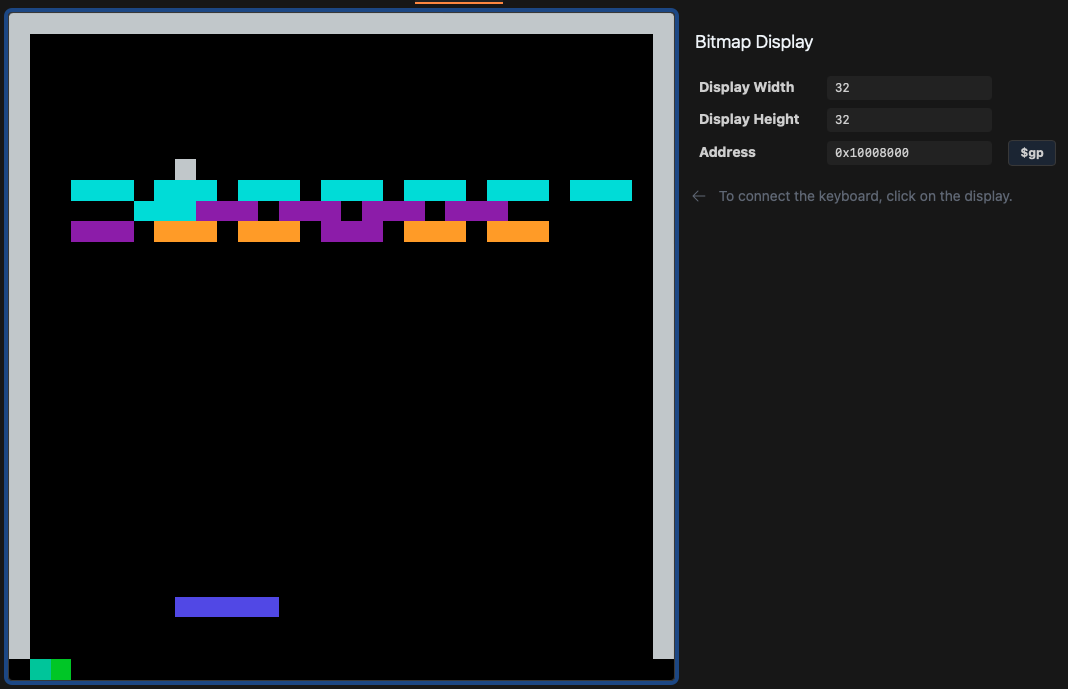
\includegraphics[width=0.6\textwidth]{static2.png}
    \caption{While Playing}
    \label{Static}
\end{figure}
\newpage
\item Game Summary:
% TODO: Tell us a little about your game.
\begin{itemize}
\item \texttt{game\_started} is a flag that is used to check if the game has started by clicking 'Spacebar'.
\item \texttt{COLOURS} are lined for the bricks, walls, paddle, ball and eraser.
\item \texttt{PADDLE\_POS} denotes the coordinates of the paddle.
\item \texttt{BALL\_POS} denotes the coordinates of the ball.
\item \texttt{BALL\_DIR} denotes the direction of the ball.
\item \texttt{BRICK\_WIDTH} denotes the brick width.
\item \texttt{BRICK\_HEIGHT} denotes the brick height.
\item “How will the ball change directions when it collides?” Depending on what side of the ball gets collided, either the 'x' or 'y' velocity will get sign flipped.
\item Paddle is 5x1.
\item 1 level with 3 rows of bricks, however only one piece of the brick breaks off at a time.
\item Ball is a 1x1 pixel for simplicity.
\item Ball currently only goes in 8 directions. Planning to add more with milestone 4-5, although walls are prone to breaking and other bugs are present when scaling the ball direction vector.
\item Note that in Figure 3 the gauge at the bottom fills up with distinguishable green pixels to indicate score tracking when any of the 20 bricks have been broken.
\item \texttt{CURR\_SCORE} keeps track of the current score.
\item \texttt{SLEEP\_RATE} denotes the time the game loop sleeps.
\end{itemize}

    
\end{enumerate}

\section{Attribution Table}
% TODO: If you worked in partners, tell us who was 
%       responsible for which features. Some reweighting 
%       might be possible in cases where one group member
%       deserves extra credit for the work they put in.

\begin{center}
\begin{tabular}{|| c | c ||}
\hline
 Student 1 (Frederick and 1006986781) &  Student 2 (Name and student number) \\ 
 \hline
 Milestone 1 & Task\\
 \hline
 Milestone 2 & Task\\
 \hline
 Milestone 3 & Task\\ 
 \hline
 Milestone 4 & Task\\ 
 \hline
 Milestone 5 & Task\\
 \hline
 Task & Task\\  
 \hline
\end{tabular}
\end{center}

% TODO: Fill out the remainder of the document as you see 
%       fit, including as much detail as you think 
%       necessary to better understand your code. 
%       You can add extra sections and subsections to 
%       help us understand why you deserve marks for 
%       features that were more challenging than they
%       might initially seem.


\end{document}
